\documentclass[]{scrartcl}

\usepackage{hyperref}
\usepackage{graphicx}
%\graphicspath{./Images/}
\usepackage{wrapfig}
\usepackage{paralist}
\usepackage{microtype}

\setlength{\parindent}{0em}
\setlength{\parskip}{1ex}

%opening
\title{Installations in Manjaro 21.2}
\author{Pablo Adames}

\begin{document}
	
	\maketitle
	
	\begin{abstract}
		Reinstalled Manjaro 21.2 on /dev/sdb following Manjaro Forum recommendations.
		Windows continues installed on /dev/sda.
		The dual boot continues to be handled well by the boot loader.
	\end{abstract}
	
	\section{Development tools}
	
	\begin{verbatim}
		sudo pacman -Syyu
		sudo pacman -S base-devel
	\end{verbatim}
	
	\section{R}
	
	\begin{verbatim}
		pamac install intel-mkl
		sudo find / -type d -iname mkl 2>/dev/null
	\end{verbatim}
	
	The output of the latter was
	\begin{verbatim}
		/opt/intel/mkl
	\end{verbatim}
	
	So I set the environment variable needed for the build step:
	
	\begin{verbatim}
		export MKLROOT="/opt/intel/mkl"
	\end{verbatim}
	
	After that the last step is:
	
	\begin{verbatim}
		pamac build r-mkl
	\end{verbatim}
	
	To find out what configuration I have:
	\begin{verbatim}
		/opt/intel/mkl/bin/mkl_link_tool
	\end{verbatim} 
	
	
	\section{RStudio}
	
	Starting from home:
	
	\begin{verbatim}
		mkdir Downloads/RStudio
		cd Downloads/RStudio
		git clone https://aur.archlinux.org/r-studio-for-linux-bin.git
		cd r-studio-for-linux-bin/
		updpkgsums
		makepkg -si	
	\end{verbatim}
	
	This is a deceivingly namesake of the real RStudio. It is a utility to manage the file system.
	Apparently there is no easy way to install RStudio in Manjaro.
	
	So I removed it from the Manjaro Software utility.
	
	Retrying:
	
	\begin{verbatim}
		mkdir Downloads/RStudio
		cd Downloads/RStudio
		git clone https://aur.archlinux.org/rstudio-desktop.git
		cd rstudio-desktop/
		updpkgsums
		makepkg -si	
	\end{verbatim}
	
	This had the error mentioned in \href{https://forum.manjaro.org/t/rstudio-on-pinebook-pro-aarch64/60827/6?u=padames}{Installing RStudio}. The responder states that the AUR repo does not have the dependencies necessary to build RStudio.
	
	\begin{figure}[!htb]
		\centering
		\caption{Error after executing \texttt{makepkg -si}}
		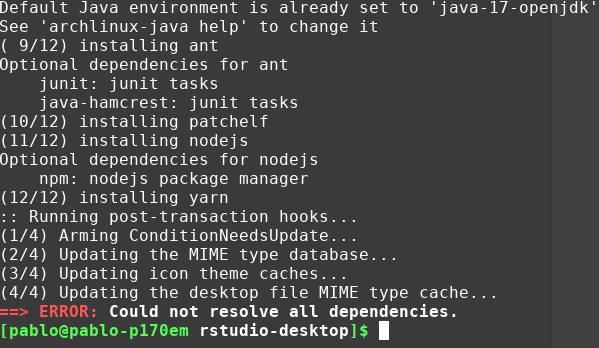
\includegraphics[width=0.45\textwidth]{Images/ErrorInstallingAUR.png}
	\end{figure}
	
	In my final attempt of the night I succeeded following the \textit{yay} route as described in \href{https://archived.forum.manjaro.org/t/using-the-statistical-package-r-in-manjaro-with-rstudio/484}{Manjaro Forum on RStudio-archived}. 
	It came down to doing a single command line:
	\begin{verbatim}
		yay -S rstudio-desktop-bin
	\end{verbatim}
	Of course, first I had to install yay (see \S\ref{sec:yay})
	
	The version installed was RStudio 2021.09.2
	
	\begin{figure}[!htb]
		\centering
		\caption{RStudio 2021.09.2 Build 382.}
		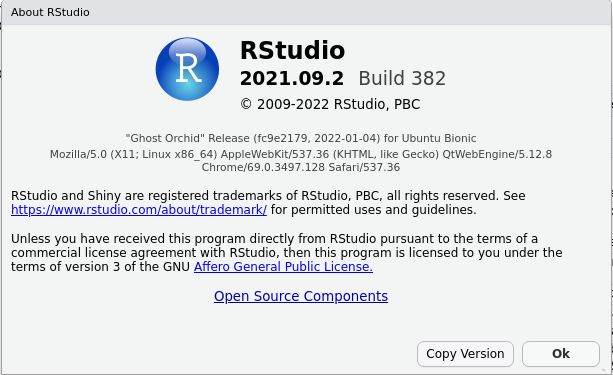
\includegraphics[width=0.45\textwidth]{Images/RStudioSplashWindowFeb07-2022.png}
	\end{figure}
	
	On October 12, 2022, I had to re-install RStudio with
	\begin{verbatim}
		yay -S rstudio-desktop-bin
	\end{verbatim}
	
	because when I tried to run RStudio there was a missing library error. 
	Re-installing seemed a reasonable solution, the package installed was rstudio-desktop-bin-2022.07.1.554-2 and \texttt{rstudio-desktop} was removed in the process.
	
	On November 16, 2022, RStudio was broken again after installing big update.
	This time I tried to solve the missing library by addressing the missing shared
	libraries libcrypto.so.1.1  and libssl.so.1.1 required by an older version of openssl.
	\href{https://stackoverflow.com/a/72366805/1585486}{libssl.so.1.1 canot open shared object SO question}
	
	\begin{tiny}
	\begin{verbatim}
		> if(!require(yaml, quietly = TRUE)) { options(Ncpus = 2 );
		    install.packages('yaml',
			                  lib='/var/tmp/pamac-build-pablo/rstudio-desktop/src/rstudio-2022.07.2-576/dependencies/R', repos='https://cran.rstudio.com/') }
		cmake: error while loading shared libraries: libssl.so.1.1: cannot open shared object file: No such file or directory
		==> ERROR: A failure occurred in build().
		Aborting...
	\end{verbatim}
	\end{tiny}


	I retried the yay installation, which uses the debian package.
	
	
	Again this installs a working version of RStudio. My take is that after updates the version of the
	openssl required libraries get removed in favour of more recent ones. 
	
	\begin{figure}[!htb]
	\centering
	\caption{RStudio 2022.07.2 Build 576 installed o Nov. 16, 2022 via Yay.}
	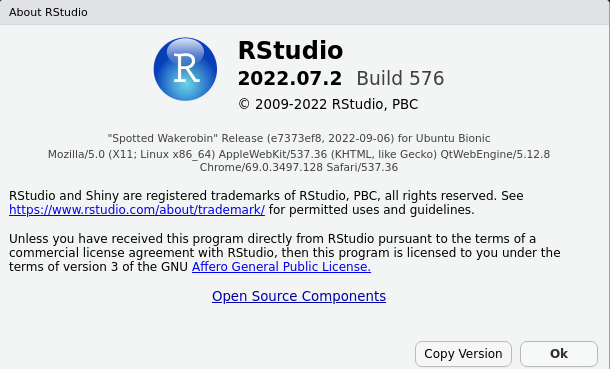
\includegraphics[width=0.45\textwidth]{Images/RStudioSplashWindowNov-16-2022.png}
	\end{figure}
	
	
	On November 22, 2022 there was no RStudio to be found when running either the kernel
	version 5.15.78-1 or the previous 5.10.136
	
	\begin{small}
		\begin{verbatim}
			[pablo@pablo-p170em ~]$ uname -srm
			Linux 5.15.78-1-MANJARO x86_64
		\end{verbatim}
	\end{small}
	
	When running the Yay installation command I saw:
	
	\begin{small}
		\begin{verbatim}
			[pablo@pablo-p170em ~]$ yay -S rstudio-desktop-bin
			:: Checking for conflicts...
			:: Checking for inner conflicts...
			[Aur:1]  rstudio-desktop-bin-2022.07.2.576-1
			
			1 rstudio-desktop-bin                      (Build Files Exist)
			...
			==> Making package: rstudio-desktop-bin 2022.07.2.576-1 (Tue 22 Nov 2022 07:05:52 AM)
			==> Checking runtime dependencies...
			==> Checking buildtime dependencies...
			==> Retrieving sources...
			-> Found rstudio-2022.07.2-576-amd64.deb
			==> Validating source_x86_64 files with sha256sums...
			rstudio-2022.07.2-576-amd64.deb ... Passed
			==> Removing existing $srcdir/ directory...
			==> Extracting sources...
			-> Extracting rstudio-2022.07.2-576-amd64.deb with bsdtar
			==> Sources are ready.
			...
			==> Leaving fakeroot environment.
			==> Finished making: rstudio-desktop-bin 2022.07.2.576-1 (Tue 22 Nov 2022 07:06:16 AM)
			==> Cleaning up...
			error: could not set install reason for package rstudio-desktop-bin 
			(could not find or read package)
		\end{verbatim}
	\end{small}
	
	So, what had succeeded a few days ago now fails!
	
	I arrived at Bryan Jenks YouTube channel where I followed the \href{https://www.youtube.com/watch?v=FhvEJxrzABI}{AUR pakage installation
	video}. Then I installed it via the \href{https://www.youtube.com/watch?v=XAId0j7RR0c}{RStudio for Arh Linux video}.
	
	The build part takes over 2 hours on the Sager laptop. It may potentially fail if there are incompatible dependencies at the 
	system level that cannot be resolved by the package manager AUR.
	
	The installation finished without errors:
	
	\begin{small}
		\begin{verbatim}
			(1/1) installing rstudio-desktop             [################################]100%
			Optional dependencies for rstudio-desktop
			git: for git support [installed]
			subversion: for subversion support
			openssh-askpass: for a git ssh access
			quarto: for Quarto projects support
			:: Running post-transaction hooks...
			(1/4) Arming ConditionNeedsUpdate...
			(2/4) Updating the MIME type database...
			(3/4) Updating icon theme caches...
			(4/4) Updating the desktop file MIME type cache...
		\end{verbatim}
	\end{small}
	
	
	Created the script \texttt{rstudio} under \textasciitilde$\backslash$.local$\backslash$bin$\backslash$tools, with the following content:
	
	\begin{small}
		\begin{verbatim}
			#!/usr/bin/env sh
			
			#open RStudio desktop from the command line
			
			/usr/bin/rstudio-bin & disown
			
			PPPID=$(awk '{print $4}' "/proc/$PPID/stat")
			kill $PPPID
			
		\end{verbatim}
	\end{small}
	
	Just clicking on the RStudio link o the task bar worked well. However the Quarto CLI component
	has a message that it needs update.
	
	Ran a \texttt{install.packages("quarto")} followed by package updates:
	
	\begin{tiny}
		\begin{verbatim}
			install.packages(c("bit", "evaluate", "knitr", "learnr", "markdown", "pkgload", "R.utils", "rmarkdown", "sass", "styler", "vctrs", "xfun"))
		\end{verbatim}
	\end{tiny}
	
	After all this, the quarto version is 1.2, however the message at start up still asks for a minimum of 0.9.2, I think I will ignore it for now.
	I ran out of time today but a full test would be to knitr a document.
	 
	
	\subsection{Quarto installation}
	
	On December 13, 2022 I addressed a meesage on the RStudio IDE telling to update the Quarto component.
	I followed the link suggested by the message: \href{https://quarto.org/docs/download/tarball.html?version=1.2.269&idPrefix=download}{quarto}.
	
	I unpacked the package to the local folder \textasciitilde$\backslash$.local$\backslash$opt 
	and made the symlink to \textasciitilde$\backslash$.local$\backslash$bin$\backslash$quarto
	
	
	\subsection{Updating RStudio}
	
	On Dec 17, 2020 I observed the following message in the Package Manager:
	
	\begin{figure}[!htb]
		\centering
		\caption{Behind RStudio 2022.07.2 Build 576.}
		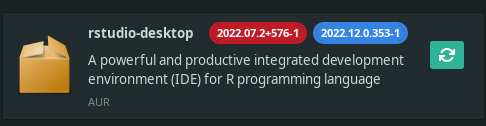
\includegraphics[width=0.45\textwidth]{Images/RStudio-failing-update-throughPckMngr.png}
	\end{figure}
	
	An indeed I am on an older version:
	\begin{tiny}
		\begin{verbatim}
			RStudio 2022.07.2+576 "Spotted Wakerobin" Release (e7373ef, 2022-11-22) for x86_64 GNU/Linux
			Mozilla/5.0 (X11; Linux x86_64) AppleWebKit/537.36 (KHTML, like Gecko) QtWebEngine/5.15.11 Chrome/87.0.4280.144 Safari/537.36
		\end{verbatim}
	\end{tiny}
	
	That is the version that got installed from the Arch repo.
	
	After viewing the videos by Brian Jenks again I realized that I installed an older version, 2022.07.2.576-1. So I looked for the  more recent version from another AUR repo because these are
	publicly maintained, \href{https://aur.archlinux.org/packages/rstudio-desktop}{rstudio-desktop}.
	
	So, step one I removed the existing version with:
	
	\begin{small}
		\begin{verbatim}
			sudo pacman -Rns rstudio-desktop	
		\end{verbatim}
	\end{small}
	
	
	The removed the directory manually.
	The next step is to clone the AUR git repo and do a makepkg in the folder.
	
	But when trying to build it there were unmet dependencies:
	
	\begin{tiny}
		\begin{verbatim}
			[pablo@pablo-p170em rstudio-desktop]$ makepkg -si
			==> Making package: rstudio-desktop 2022.12.0.353-1 (Sat 17 Dec 2022 07:57:15 PM)
			==> Checking runtime dependencies...
			==> Installing missing dependencies...
			[sudo] password for pablo: 
			error: target not found: soci
			==> ERROR: 'pacman' failed to install missing dependencies.
			==> Missing dependencies:
			-> qt5-sensors
			-> qt5-xmlpatterns
			-> postgresql-libs
			-> soci
			-> mathjax2
			-> pandoc
			-> yaml-cpp
			==> Checking buildtime dependencies...
			==> ERROR: Could not resolve all dependencies.
		\end{verbatim}
	\end{tiny}
	
	On Dec 18 I did a refresh of yay with
	\begin{small}
		\begin{verbatim}
			sudo pacman -S --needed git base-devel yay	
	    \end{verbatim}
	\end{small}
	yay-git was removed and then the update above went away (?). Got the same error after cloning and running 
	\begin{verbatim}
		makepkg -si
	\end{verbatim}
	
	So the best path now is to try to resolve the missing dependencies.
	
	Executing:
	
	\begin{small}
		\begin{verbatim}
			pamac install qt5-sensors
			pamac install qt5-xmlpatterns
			pamac install postgresql-libs
			pamac install mathjax2
			pamac install pandoc
			pamac install yaml-cpp
		\end{verbatim}
	\end{small}
	
	For soci, the C++ compliant Object Database Library interface, I followed the download and build from source istructions in \href{https://soci.sourceforge.net/doc/master/installation/}{soci}.
	
	Basically cloning with 
	
	\begin{tiny}
		\begin{verbatim}
			 $ git clone https://github.com/SOCI/soci.git
			 $ cd soci
			 $ mkdir build && cd build
			 $ cmake -G ``Unix Makefiles'' -DWITH\_BOOST=OFF -DWITH\_ORACLE=OFF  \~{}/Programs/soci/
			 ...
			 -- Configuring SOCI: 
			 -- SOCI\_VERSION                             = 4.1.0 
			 -- SOCI\_ABI\_VERSION                         = 4.1 
			 -- SOCI\_SHARED                              = ON 
			 -- SOCI\_STATIC                              = ON 
			 -- SOCI\_TESTS                               = ON 
			 -- SOCI\_ASAN                                = OFF 
			 -- LIB\_SUFFIX                               = 64 
			 ...
			 -- MySQL: 
			 -- Performing Test HAVE_MYSQL_OPT_EMBEDDED_CONNECTION
			 -- Performing Test HAVE_MYSQL_OPT_EMBEDDED_CONNECTION - Failed
			 -- MySQL not found.
			 -- MySQL Embedded not found.
			 -- WARNING: MySQL libraries not found, some features will be disabled. 
			 -- ODBC: 
			 -- ODBC_INCLUDE_DIR                         = /usr/include 
			 -- ODBC_LIBRARIES                           = /usr/lib/libodbc.so 
			 -- Oracle: disabled, since WITH_ORACLE=OFF 
			 -- PostgreSQL: 
			 -- POSTGRESQL_INCLUDE_DIRS                  = /usr/include 
			 -- POSTGRESQL_LIBRARIES                     = /usr/lib/libpq.so 
			 -- POSTGRESQL_VERSION                       = 14.6 
			 -- SQLite3: 
			 -- SQLITE3_INCLUDE_DIR                      = /usr/include 
			 -- SQLITE3_LIBRARIES                        = /usr/lib/libsqlite3.so 
			 ...
			 -- PostgreSQL - SOCI backend for PostgreSQL 
			 -- SOCI_POSTGRESQL                          = ON 
			 -- SOCI_POSTGRESQL_TARGET                   = soci_postgresql 
			 -- SOCI_POSTGRESQL_OUTPUT_NAME              = soci_postgresql 
			 -- SOCI_POSTGRESQL_COMPILE_DEFINITIONS      = SOCI_ABI_VERSION="4.1" HAVE_DL=1 
			 -- SOCI_POSTGRESQL_INCLUDE_DIRECTORIES      = /home/pablo/Programs/soci/build /home/pablo/Programs/soci/include /home/pablo/Programs/soci/build/include /home/pablo/Programs/soci/include/private /home/pablo/Programs/soci/include/private /usr/include /usr/include 
			 -- SOCI_POSTGRESQL_NOSINLGEROWMODE          =  
			 ...
			 -- Configuring done
			 -- Generating done
			 -- Build files have been written to: /home/pablo/Programs/soci/build
			 $ make
			 ...
			 [  0%] Building CXX object src/core/CMakeFiles/soci_core.dir/backend-loader.cpp.o
			 [  1%] Building CXX object src/core/CMakeFiles/soci_core.dir/blob.cpp.o
			 [  1%] Building CXX object src/core/CMakeFiles/soci_core.dir/common.cpp.o
			 ...
			 [ 94%] Linking CXX executable ../../bin/soci_odbc_test_postgresql
			 [ 94%] Built target soci_odbc_test_postgresql
			 [ 95%] Building CXX object tests/odbc/CMakeFiles/soci_odbc_test_postgresql_static.dir/test-odbc-postgresql.cpp.o
			 [ 95%] Linking CXX executable ../../bin/soci_odbc_test_postgresql_static
			 [ 95%] Built target soci_odbc_test_postgresql_static
			 [ 95%] Building CXX object tests/postgresql/CMakeFiles/soci_postgresql_test.dir/test-postgresql.cpp.o
			 [ 96%] Linking CXX executable ../../bin/soci_postgresql_test
			 [ 96%] Built target soci_postgresql_test
			 [ 97%] Building CXX object tests/postgresql/CMakeFiles/soci_postgresql_test_static.dir/test-postgresql.cpp.o
			 [ 97%] Linking CXX executable ../../bin/soci_postgresql_test_static
			 [ 97%] Built target soci_postgresql_test_static
			 [ 98%] Building CXX object tests/sqlite3/CMakeFiles/soci_sqlite3_test.dir/test-sqlite3.cpp.o
			 [ 98%] Linking CXX executable ../../bin/soci_sqlite3_test
			 [ 98%] Built target soci_sqlite3_test
			 [ 99%] Building CXX object tests/sqlite3/CMakeFiles/soci_sqlite3_test_static.dir/test-sqlite3.cpp.o
			 [100%] Linking CXX executable ../../bin/soci_sqlite3_test_static
			 [100%] Built target soci_sqlite3_test_static
			 $ sudo make install
			 [ 14%] Built target soci_core
			 [ 28%] Built target soci_core_static
			 [ 35%] Built target soci_empty
			 [ 42%] Built target soci_empty_static
			 [ 49%] Built target soci_odbc
			 [ 55%] Built target soci_odbc_static
			 [ 63%] Built target soci_postgresql
			 [ 70%] Built target soci_postgresql_static
			 ...
			 -- Set runtime path of "/usr/local/lib/libsoci_odbc.so.4.1.0" to ""
			 -- Installing: /usr/local/lib/libsoci_odbc.so
			 -- Installing: /usr/local/lib/libsoci_odbc.a
			 -- Installing: /usr/local/include/soci/postgresql/soci-postgresql.h
			 -- Installing: /usr/local/lib/libsoci_postgresql.so.4.1.0
			 -- Installing: /usr/local/lib/libsoci_postgresql.so.4.1
			 -- Set runtime path of "/usr/local/lib/libsoci_postgresql.so.4.1.0" to ""
			 -- Installing: /usr/local/lib/libsoci_postgresql.so
			 -- Installing: /usr/local/lib/libsoci_postgresql.a
			 -- Installing: /usr/local/include/soci/sqlite3/soci-sqlite3.h
			 -- Installing: /usr/local/lib/libsoci_sqlite3.so.4.1.0
			 -- Installing: /usr/local/lib/libsoci_sqlite3.so.4.1
			 -- Set runtime path of "/usr/local/lib/libsoci_sqlite3.so.4.1.0" to ""
			 -- Installing: /usr/local/lib/libsoci_sqlite3.so
			 -- Installing: /usr/local/lib/libsoci_sqlite3.a
		\end{verbatim}
	\end{tiny} 
	
	I removed the dependency on soci manually from the PKGBUILD file because installig soci the way I did does<not install a system package but only libraries under |/usr/local/lb|.
	
	I had to add the following to the cmake section of he PKGBUILD file to use C++17 and avoid some errors I saw while compiling with default values.
	
	\begin{tiny}
		\begin{verbatim}
			-DCMAKE_CXX_STANDARD=17 \
			-DCMAKE_CXX_STANDARD_REQUIRED=ON \
			-DCMAKE_CXX_EXTENSIONS=OFF \
		\end{verbatim}
	\end{tiny}
	
	The build failed because I don't have headers for openssl, in particular the declaration of the function
	
	\begin{tiny}
		\begin{verbatim}
			src/node-v16.14.0-linux-x64/include/node/openssl/evp.h:996:int EVP_PKEY_size(const EVP_PKEY *pkey);
			
		\end{verbatim}
	\end{tiny}
	
	The function is defined in the openssl file \verb|crypto/evp/p_lib.c| that I foud in the source code I clones by
	
	\begin{small}
		\begin{verbatim}
			git clone git://git.openssl.org/openssl.git
		\end{verbatim}
	\end{small}
	
	Eve after this I stop now at 53\% build with no obvious compiler errors while linking object file \verb|src/cpp/desktop/CMakeFiles/rstudio.dir/qrc_desktop.cpp.o|
	
	This is too much work to install a more recent RStudio  my opinion. It has been fun but very hard and no result to show.
	
	
	Going back to investigate to the AUR web page for rstudio I found that the soci dependency is on an AUR package called \texttt{soci-git}. 
	This is different from the source that I installed straight from git but generic for any linux system.
	
	\begin{scriptsize}
		\begin{verbatim}
			1. git clone https://aur.archlinux.org/soci-git.git
			2. cd soci-git
			3. vim PKGBUILD
			4. makepkg -si
			
		\end{verbatim}
	\end{scriptsize}

	It fails making the package:
	
	\begin{tiny}
		\begin{verbatim}
			 52%] Building CXX object src/cpp/desktop/CMakeFiles/rstudio.dir/synctex/evince/moc_EvinceWindow.cpp.o
			[ 52%] Building CXX object src/cpp/desktop/CMakeFiles/rstudio.dir/qrc_desktop.cpp.o
			[ 52%] Linking CXX executable rstudio
			make[2]: Leaving directory '/home/pablo/Programs/rstudio-desktop/src/build'
			[ 58%] Built target rstudio
			make[1]: Leaving directory '/home/pablo/Programs/rstudio-desktop/src/build'
			make: *** [Makefile:156: all] Error 2
			make: Leaving directory '/home/pablo/Programs/rstudio-desktop/src/build'
			==> ERROR: A failure occurred in package().
			Aborting...
			
		\end{verbatim}
	\end{tiny}
	
	I am giving up for this weekend on RStudio for Manjaro
	
	
	
	\section{Yay}
	\label{sec:yay}
	
	Followed directions from \href{https://www.tecmint.com/install-yay-aur-helper-in-arch-linux-and-manjaro/}{Installing Yay}
	
	\section{AUR}
	
	Enabled AUR in the Add/Remove Software to have access to the Arch Liux packages in Manjaro as suggested \href{https://forum.manjaro.org/t/dropbox-install-new-to-manjaro/9576/5}{here} while searching for a recipe to install Dropbox.
	
	\section{Date}
	
	On April, 17, 2022 Manjaro reported the wrong date after installing updates.
	Followed these steps to fix it (\href{https://archived.forum.manjaro.org/t/howto-get-your-time-timezone-right-using-manjaro-windows-dual-boot/89359}{get your time zone}):
	\begin{compactenum}
		\item  \verb|sudo timedatectl set-local-rtc 0|
		\item \verb|sudo systemctl enable --now systemd-timesyncd|
		\item \verb|sudo ln -sf /usr/share/zoneinfo/Canada/Mountain /etc/localtime|
	\end{compactenum}
	
	The region and time zone were found by first printing out all the time zones with:
	
	\verb|find /usr/share/zoneinfo/ -maxdepth 1 -type d|
	
	sample output:
	
	\begin{verbatim}
		/usr/share/zoneinfo/
		/usr/share/zoneinfo/Antarctica
		/usr/share/zoneinfo/Indian
		/usr/share/zoneinfo/Atlantic
		/usr/share/zoneinfo/America
		/usr/share/zoneinfo/Europe
		/usr/share/zoneinfo/Africa
		/usr/share/zoneinfo/Asia
		/usr/share/zoneinfo/Canada
		/usr/share/zoneinfo/right
		/usr/share/zoneinfo/Brazil
		/usr/share/zoneinfo/Arctic
		/usr/share/zoneinfo/Mexico
		/usr/share/zoneinfo/Chile
		/usr/share/zoneinfo/Pacific
		/usr/share/zoneinfo/Etc
		/usr/share/zoneinfo/Australia
		/usr/share/zoneinfo/US
		/usr/share/zoneinfo/posix
	\end{verbatim}
	
	Then the Canadian time zones with:
	
	\verb|ls /usr/share/zoneinfo/Canada|
	
	The output was:
	
	\begin{verbatim}
		Atlantic  Eastern   Newfoundland  Saskatchewan
		Central   Mountain  Pacific       Yukon
	\end{verbatim}
	
	This fixed my time zone issue today! Check with the command \texttt{date}.
	
	\section{Dropbox}
	
	Followed the \href{https://forum.manjaro.org/t/dropbox-install-new-to-manjaro/9576/5}{page in Manaro Forum}.
	
	First attempt here failed:
	\begin{small}
		\begin{verbatim}
			-> Downloading dropbox-lnx.x86_64-139.4.4896.tar.gz...
			% Total    % Received % Xferd  Average Speed   Time    Time     Time  Current
			Dload  Upload   Total   Spent    Left  Speed
			
			0     0    0     0    0     0      0      0 --:--:-- --:--:-- --:--:--     0
			2 96.1M    2 2578k    0     0  2757k      0  0:00:35 --:--:--  0:00:35 2755k
			9 96.1M    9 9310k    0     0  4804k      0  0:00:20  0:00:01  0:00:19 4804k
			16 96.1M   16 15.8M    0     0  5526k      0  0:00:17  0:00:02  0:00:15 5525k
			23 96.1M   23 22.6M    0     0  5890k      0  0:00:16  0:00:03  0:00:13 5888k
			30 96.1M   30 29.6M    0     0  6144k      0  0:00:16  0:00:04  0:00:12 6143k
			37 96.1M   37 36.2M    0     0  6248k      0  0:00:15  0:00:05  0:00:10 6900k
			44 96.1M   44 43.2M    0     0  6381k      0  0:00:15  0:00:06  0:00:09 6992k
			52 96.1M   52 50.2M    0     0  6484k      0  0:00:15  0:00:07  0:00:08 7048k
			59 96.1M   59 57.1M    0     0  6550k      0  0:00:15  0:00:08  0:00:07 7070k
			66 96.1M   66 63.7M    0     0  6566k      0  0:00:14  0:00:09  0:00:05 6982k
			73 96.1M   73 70.4M    0     0  6600k      0  0:00:14  0:00:10  0:00:04 7020k
			80 96.1M   80 77.5M    0     0  6657k      0  0:00:14  0:00:11  0:00:03 7040k
			87 96.1M   87 84.2M    0     0  6671k      0  0:00:14  0:00:12  0:00:02 6968k
			94 96.1M   94 90.9M    0     0  6685k      0  0:00:14  0:00:13  0:00:01 6927k
			100 96.1M  100 96.1M    0     0  6711k      0  0:00:14  0:00:14 --:--:-- 7017k
			-> Downloading dropbox-lnx.x86_64-139.4.4896.tar.gz.asc...
			% Total    % Received % Xferd  Average Speed   Time    Time     Time  Current
			Dload  Upload   Total   Spent    Left  Speed
			
			0     0    0     0    0     0      0      0 --:--:-- --:--:-- --:--:--     0
			100   473  100   473    0     0   2544      0 --:--:-- --:--:-- --:--:--  2556
			==> Validating source files with sha256sums...
			DropboxGlyph_Blue.svg ... Passed
			terms.txt ... Passed
			dropbox.service ... Passed
			dropbox@.service ... Passed
			==> Validating source_x86_64 files with sha256sums...
			dropbox-lnx.x86_64-139.4.4896.tar.gz ... Passed
			dropbox-lnx.x86_64-139.4.4896.tar.gz.asc ... Skipped
			==> Verifying source file signatures with gpg...
			dropbox-lnx.x86_64-139.4.4896.tar.gz ... FAILED (unknown public key FC918B335044912E)
			==> ERROR: One or more PGP signatures could not be verified!
			Failed to build dropbox
		\end{verbatim}
	\end{small}
	
	Second attempt was not what I expected because the installed program only opened a link to the Dropbox webpage.
	The I followed the download and build instructions from \href{https://help.dropbox.com/installs-integrations/desktop/linux-commands}{here}. 
	Then linked it to my free account which allows only three devices.
	
	\begin{figure}[!htb]
		\centering
		\caption{Connecting Dropbox client with server in the cloud. Removed the old reference to the previous Manjaro installation.}
		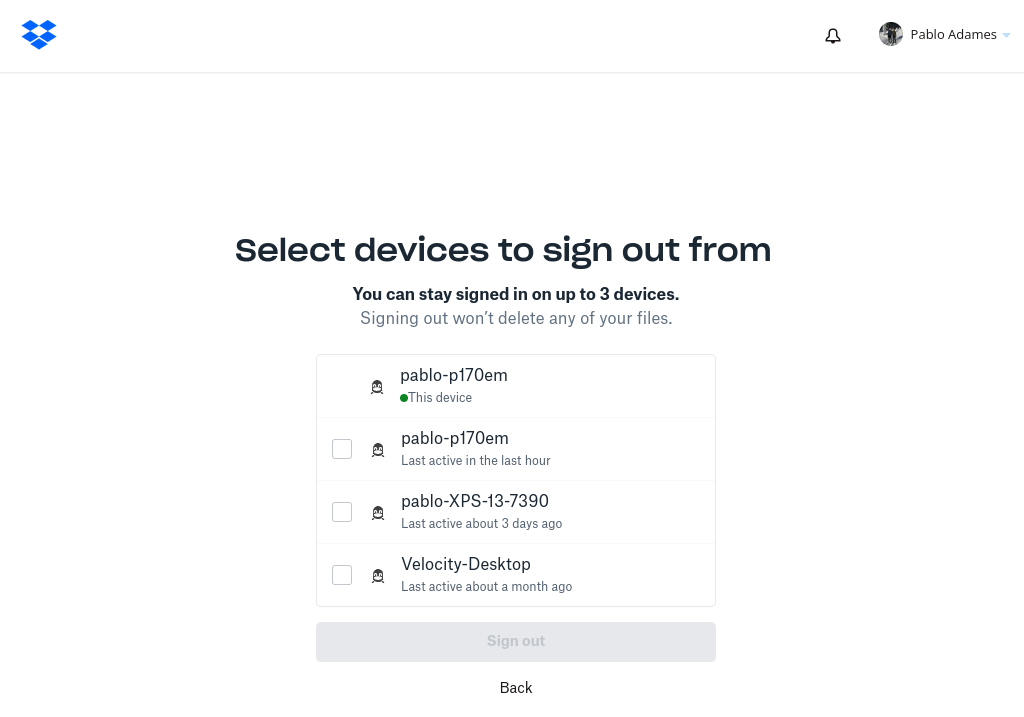
\includegraphics[width=0.8\textwidth]{Images/DropBoxSetUp.png}
	\end{figure}
	
\section{\TeX{}Live}

To install \TeX{}Live I followed the following steps:

\begin{compactenum}
	\item cloned the AUR git repo: \href{https://aur.archlinux.org/packages/texlive-full}{AUR-TeXLive}
	\item cd into the cloned project and run \texttt{makepkg} (see \href{https://wiki.archlinux.org/title/Makepkg}{Makepkg documentation})
	\item run \texttt{makepkg --install}
	\item entered password to complete the installation (if one leaves the lengthy installation unattended it may time out while waiting for the user password)
\end{compactenum}


\section{\TeX{}Studio}

Simply ran \texttt{sudo pamac install texstudio} at the command line.
See more information in the Manjaro page  \href{https://software.manjaro.org/package/texstudio}{\TeX{}Studio Manjaro}.


\section{Calibre}

Followed the download and installation instructions in \href{https://calibre-ebook.com/download_linux}{Calibre}.

\begin{footnotesize}
	\begin{verbatim}
		sudo -v && wget -nv -O- https://download.calibre-ebook.com/linux-installer.sh | sudo sh /dev/stdin
	\end{verbatim}
\end{footnotesize}


	
\end{document}
